\documentclass[12pt, a4paper]{article}
\usepackage[czech]{babel}
\usepackage[utf8]{inputenc}
\usepackage{tabularx}
\usepackage[left=2cm,text={17cm, 24cm},top=3cm]{geometry}
\usepackage[unicode]{hyperref}
\usepackage{graphicx}


\begin{document}
    \begin{titlepage}
        \begin{center}
            {\Huge
            \textsc{Vysoké učení technické v Brně}}\\
            {\huge \textsc{Fakulta informačních technologií}\\
            \vspace{\stretch{0.900}}}
            {\LARGE
            Konvoluční neuronové sítě -- Semestrální projekt}\\
            {\Huge Obarvování obrazu\\
            \vspace{250pt}}

            {\Large
            \begin{center}
                \begin{minipage}[b]{0.33333\textwidth}
                    \raggedright
                    Tomáš Venkrbec \par
                    \href{mailto:xvenkr01@vutbr.cz}{xvenkr01@vutbr.cz} 
                \end{minipage}%
                \begin{minipage}[b]{0.33333\textwidth}
                    \centering
                    Kateřina Fořtová \par
                    \href{mailto:xforto00@vutbr.cz}{xforto00@vutbr.cz}
                \end{minipage}%
                \begin{minipage}[b]{0.33333\textwidth}
                    \raggedleft
                    Jiří Dvořák \par
                    \href{mailto:xdvora2u@vutbr.cz}{xdvora2u@vutbr.cz}
                \end{minipage}
            \end{center}}

            \vspace{30pt}
            {\Large \today}
            \vspace{\stretch{0.100}}
        \end{center}
    \end{titlepage}
    
    \section{Popis problému}
    Zadáním projektu bylo vytvoření modelu schopného provádět automatické obarvování obrazu. Tím rozumíme úlohu přidání barev do šedotónového obrazu bez nutných zásahů uživatele. Tato úloha je ze své podstaty obecně nejednoznačná a konkrétní výstup tak záleží na dodatečných informacích, kontextu či vzorových datech. Naším cílem bylo vyvinout model využívající generativních neuronových sítí (GAN), který dokáže obarvit snímky s rozličnými typy objektů, jak snímky z námi zvoleného datasetu, tak snímky nahrané uživatelem. 
    
    \section{Analýza existujícího řešení -- DeOldify}
    DeOldify \cite{deoldify} je open-source model hlubokého učení, jehož první verzi implementoval Jason Antic již mezi lety 2018 a 2019. Cílem bylo vytvoření modelu pro obarvování historických šedotónových snímků. Model vychází převážně z modelu SAGAN, který oproti vanilla verzi GAN dokáže při trénování zahrnout kontext z celé plochy obrázku, nikoliv pouze z lokálního okolí. Zároveň je model inspirovaný principem modelu Progressive Growing GAN, který umožňuje dosáhnout vyššího rozlišení snímků. Generátor využívá architekturu sítě U-Net, která byla původně vyvinuta pro segmentaci biomedicínských dat, ale lze jí  využít i pro tento účel. V dnešní době se DeOldify více zaměřuje na obarvování videa, námi implementovaný model se inspiroval starší verzí\footnote{\url{https://github.com/dana-kelley/DeOldify}}, která pracovala pouze s obarvováním šedotónových fotografií.
    
    \section{Dataset}
    
    \subsection{ImageNet}\label{section:ImageNet}
    ImageNet\footnote{\url{https://www.image-net.org/about.php}} je datovou sadou čítající přes milion a čtvrt snímků zařazených do 1000 kategorií \cite{ImageNetStats}. Jedná se o jednu z nejznámějších datových sad využívanou zejména v úlohách strojového učení. Veliká rozličnost snímků mnoha různých objektů přináší ovšem jistou nevýhodu při trénování námi implementovaného modelu, protože trénování probíhá déle a nedosahuje tak kvalitních výsledků, než kdyby se využívalo pouze určité podkategorie snímků (např. snímky přírody nebo obličejů). Pro trénování byla využita verze datasetu se snímky rozměrů 64 $\times$ 64 pixelů.
    
    \subsection{COCO dataset}
    Ve své práci jsme se rozhodli provést experimenty i s dalším datasetem. Jedná se o COCO dataset\footnote{\url{https://cocodataset.org/##home}}, který obsahuje více jak 328 tisíc snímků zařazených do 91 objektových kategorií \cite{lin2015microsoft}. Každý objekt je poté i zařazen do nadtřídy -- např. objekty \textit{bicycle}, \textit{car}, \textit{motorcycle}, \textit{airplane}, \textit{bus}, \textit{train}, \textit{truck} nebo \textit{boat} jsou zařazeny do nadřídy \textit{vehicle} \cite{CocoCategories}. COCO dataset jsme se rozhodli využít zvláště z důvodu snadné možnosti vybrání pouze několika kategorií obrázků, protože dataset ImageNet je příliš rozsáhlým a obsahuje obrovské množství rozličných objektů. Při trénování jsme využili jak rozlišení 64 $\times$ 64, tak i vyššího rozlišení 128 $\times$ 128 pixelů.
    
    \section{Řešení}
    Kromě skriptů obsahující implementace \textit{self-attention}\footnote{\url{https://github.com/kiyohiro8/SelfAttentionGAN}} vrstvy a \textit{spektrální normalizace}\footnote{\url{https://github.com/IShengFang/SpectralNormalizationKeras}} je celá implementace řešení již pouze naší prací, nepřejímáme žádné již existující řešení. 
    
    \subsection{Implementační detaily}
    Projekt byl implementován v jazyce Python, k implementaci modelů neuronových sítí byla využita knihovna \textit{Tensorflow}, přesněji její rozhraní \textit{Keras}. Ke zjednodušení procesu evaluace byl k vizualizaci všech relevantních trénovacích metrik využit nástroj \textit{Tensorboard}.
    
    \subsection{Spouštěcí skript}
    Veškerá práce s vytvořenou neuronovou sítí je iniciována centrálně ze skriptu \texttt{run.py}. Je umožněno spustit trénování neuronové sítě od počátku, pokračovat v trénování po načtení již dříve natrénovaných vah a nebo pouze překonvertovat vlastní černobílé obrázky pomocí natrénované sítě.
    
    Ke konverzi vlastních snímků je třeba spustit skript s argumentem \texttt{--images}, k pokračování dřívějšího trénování slouží argument \texttt{--load\_weights} a základní chování bez použití argumentů je trénování modelu od počátku. Rovněž nastavitelné jsou veškeré cesty k vstupům a výstupům a většina parametrů nastavení sítě a trénování. Popis všech argumentů lze najít použitím argumentu \texttt{--help}.
    
    \subsection{Model}
    Naše řešení, stejně jako DeOldify, kterým jsme byli inspirováni, používá Self-Attention GAN \cite{sagan}, zkráceně SAGAN.
    
    \subsubsection{Diskriminátor}
    Diskriminátor je z dvojice sítí tou jednodušší, jedná se o klasickou konvoluční neuronovou síť využívající architekturu VGG. V každém konvolučním bloku, sestávajícím se z dvou konvolučních vrstev, využíváme za každou konvoluční vrstvou spektrální normalizaci a aktivační funkci \textit{LeakyReLU}. Self-attention blok přidáváme pouze jednou do celé sítě, a to na konec bloku s rozlišením 32 $\times$ 32. Použití právě při tomto rozlišení je podle autorů této techniky nejefektivnější \cite{sagan}. Diskriminátor je trénován tradičně pomocí optimalizátoru \textit{Adam} s koeficientem učení $0.0004$. Vstupem této sítě jsou tedy barevné obrázky a výstupem je pravděpodobnost, zda se jedná o skutečný či falešný obrázek.
    
    \subsubsection{Generátor}
    Zajímavější částí generativních sítí je generátor. Tuto síť jsme vytvořili podle U-Net architektury, která je kromě segmentace, ke které byla původně vytvořená, vhodná i na úlohy jako \textit{Image-to-image Translation} a \textit{Super-resolution} a proto jí lze použít i na řešení tohoto problému. 
    
    Konvoluční bloky v generátoru jsou podobné těm v diskriminátoru, pro každé rozlišení máme dvojici konvolučních vrstev se spektrálními normalizacemi. Čím je architektura speciální je práce s výstupy těchto konvolučních bloků. Jak je na obrázku \ref{unet} vidět, výstupy bloků jsou vstupy nejen dalších bloků se sníženým rozlišením, ale jsou také kopírovány na druhou stranu sítě do \textit{upscaling} části sítě, na vstup bloku se stejným rozlišením, jako je rozlišení výstupu.
    
    \begin{figure}
        \centering
        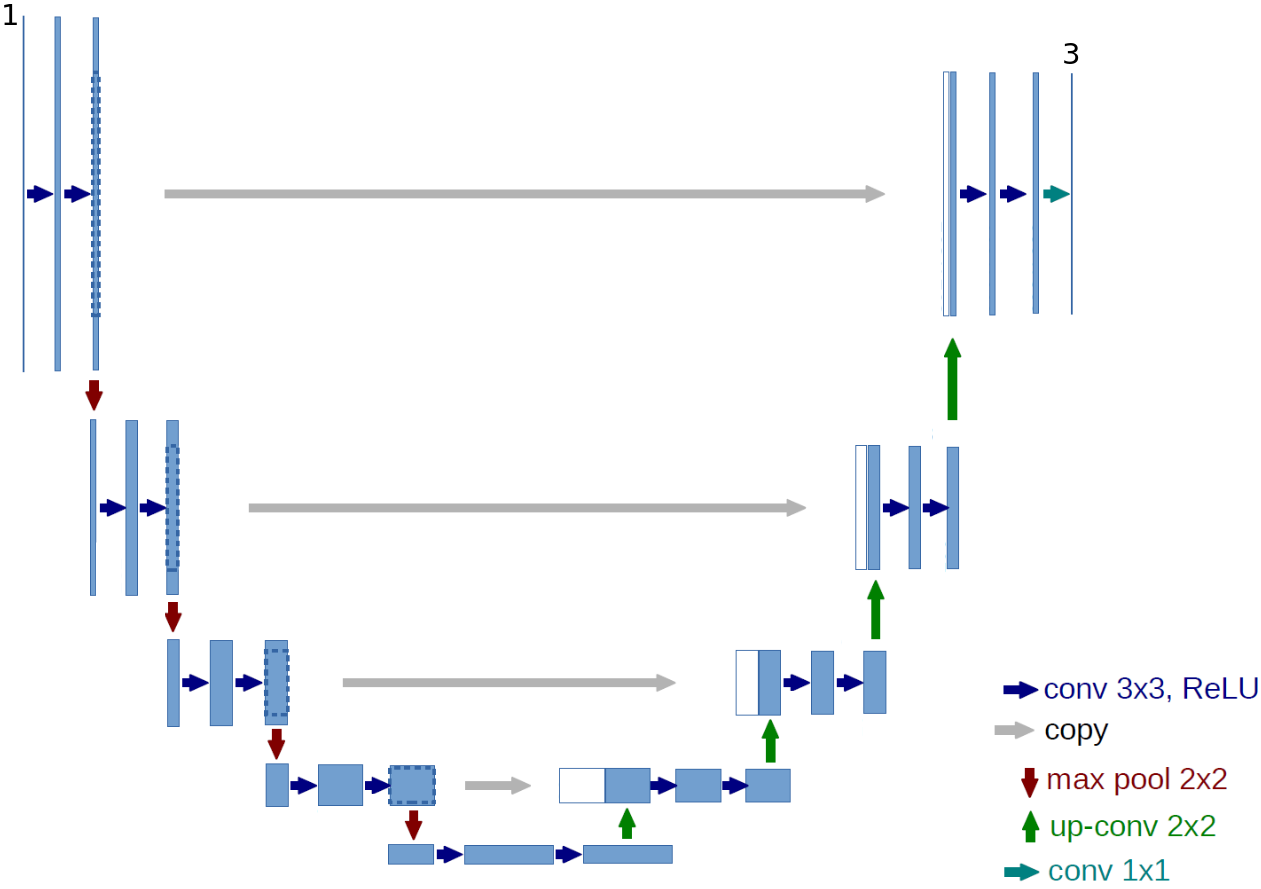
\includegraphics[width=300pt]{unet.png}
        \caption{Architektura U-Net použitá v generátoru}
        \label{unet}
    \end{figure}
    
    Rovněž podobné je využití self-attention bloků, které jsou opět využity v blocích s rozlišením 32 $\times$ 32 pixelů, a to jak v downscaling, tak v upscaling části neuronové sítě. Výstupem upscaling části sítě je obarvený vstupní šedotónový obrázek. 
    
    Generátor je také trénován pomocí optimalizátoru \textit{Adam}, ovšem s menším koeficientem učení oproti diskriminátoru, a to $0.0001$. Toto se používá ke stabilizaci a urychlení trénování sítí, jelikož je to alternativou více trénovacích kroků diskriminátoru než generátoru \cite{ttur}. 
    
    \subsubsection{Chybové funkce}
    Diskriminátor se učí rozpoznávat původ obrázků -- zda pochází z datové sady, nebo jsou výstupy generátoru. U vstupních obrázků tyto informace vždy máme, tudíž můžeme jako chybovou funkci využít \textit{Binary Cross Entropy} mezi labely vstupných dat a labely, které byly na výstupu diskriminátoru.
    
    Generátor využívá dvojici chybových funkcí. Za prvé, jelikož používáme generativní neuronové sítě a máme diskriminátor, máme chybovou funkci \textit{Adversarial Loss}. Generátor se učí tím, že se snaží co nejvíce zvýšit hodnotu chybové funkce diskriminátoru. Toto motivuje generátor k tomu, aby co nejlépe obarvoval snímky, které má na vstupu.
    Aby obarvené snímky odpovídaly obsahem těm, které jsou na vstupu, využíváme \textit{Perceptual Loss} (též známý jako \textit{Feature Loss} nebo \textit{VGG Loss}), který porovnává hodnoty aktivací ve vybraných vrstvách předtrénované VGG sítě, když je jí na vstup dán vstupní a výstupní obrázek generátoru.
    Kombinace těchto chybových funkcí motivuje generátor k tomu, aby neměnil obsah vstupního obrázku, ale pouze ho obarvil.
    
    \subsubsection{Trénování a vyhodnocování}
    Trénování probíhalo v prostředí \textit{Google Colab}, který jsme vzhledem k velikosti modelu a z ní vycházející náročnosti trénování byli nuceni použít. Trénování bylo tedy omezeno po dobu, po kterou jsou dostupné zdarma grafické karty, což se odráží na finálních výsledcích. 
    
    Pro lepší kontrolu nad procesem trénování a vyhodnocování jsme předefinovali funkce \texttt{train\_step} a \texttt{test\_step}, kterými knihovna \textit{Keras} vykonává jednotlivé kroky trénování a validace ve funkci \texttt{fit}. Díky tomu jsme mohli ručně počítat hodnoty chybových funkcí a aktualizovat váhy obou sítí. Také jsme snadněji mohli přidat vlastní callbacky k průběžnému ukládání vah modelu, vygenerovaných obrázků a všech trénovacích metrik do \textit{Tensorboard}.
    
    \section{Výsledky}
    Při trénování modelu jsme využili 3 přístupy. Nejprve byl model natrénovaný pouze na datasetu ImageNet (viz Sekce \ref{section:ImageNet}). Rozsáhlost datasetu však přinesla několik problémů, kdy trénování trvalo delší dobu a přesto nedosahovalo dobrých výsledků. Zdá se, že model má při velmi rozličných snímcích problém s velkou variancí a neví jaké rysy se přesně naučit. Proto jsme se rozhodli otestovat výsledky modelu, pokud po natrénování modelu na ImageNetu dotrénujeme tento model na specifičtější části COCO datasetu.
    
    \subsection{ImageNet}\label{results:imagenet}
    
    \subsection{COCO dataset}\label{results:coco}
    
    \subsection{Kombinované trénování}\label{results:combine}
    
    
    
    \section{Závěr}
    
    \newpage
    \bibliographystyle{czplain}
    \bibliography{bib-list}
    
\end{document}


